\documentclass[12pt]{article}

\usepackage{xcolor}
\usepackage{listings}
\usepackage{hyperref}
\usepackage{pdfpages}

\hypersetup{
    colorlinks=true,
    linkcolor=blue,
    filecolor=magenta,      
    urlcolor=cyan,
    pdftitle={HW04},
    pdfpagemode=FullScreen,
    }
\lstset{basicstyle=\ttfamily,
showstringspaces=false,
commentstyle=\color{red},
keywordstyle=\color{blue}
}

\renewcommand{\thesubsection}{\thesection.\alph{subsection}}

\title{Programming Assignment 4 \\ \small{ECE 759, Prof. TW Huang}}
\author{Sai Tadinada}
\date{}

\begin{document}
\maketitle

% TODO: Change URL!!
GitHub link to programming tasks: \\ \url{https://github.com/phantom3012/repo759/tree/main/HW04}

\section{Question 1}
\subsection{}
Installed the matplotlib library using the command: \texttt{pip install matplotlib}.
\subsection{}
\begin{figure}[ht]
    \centering
    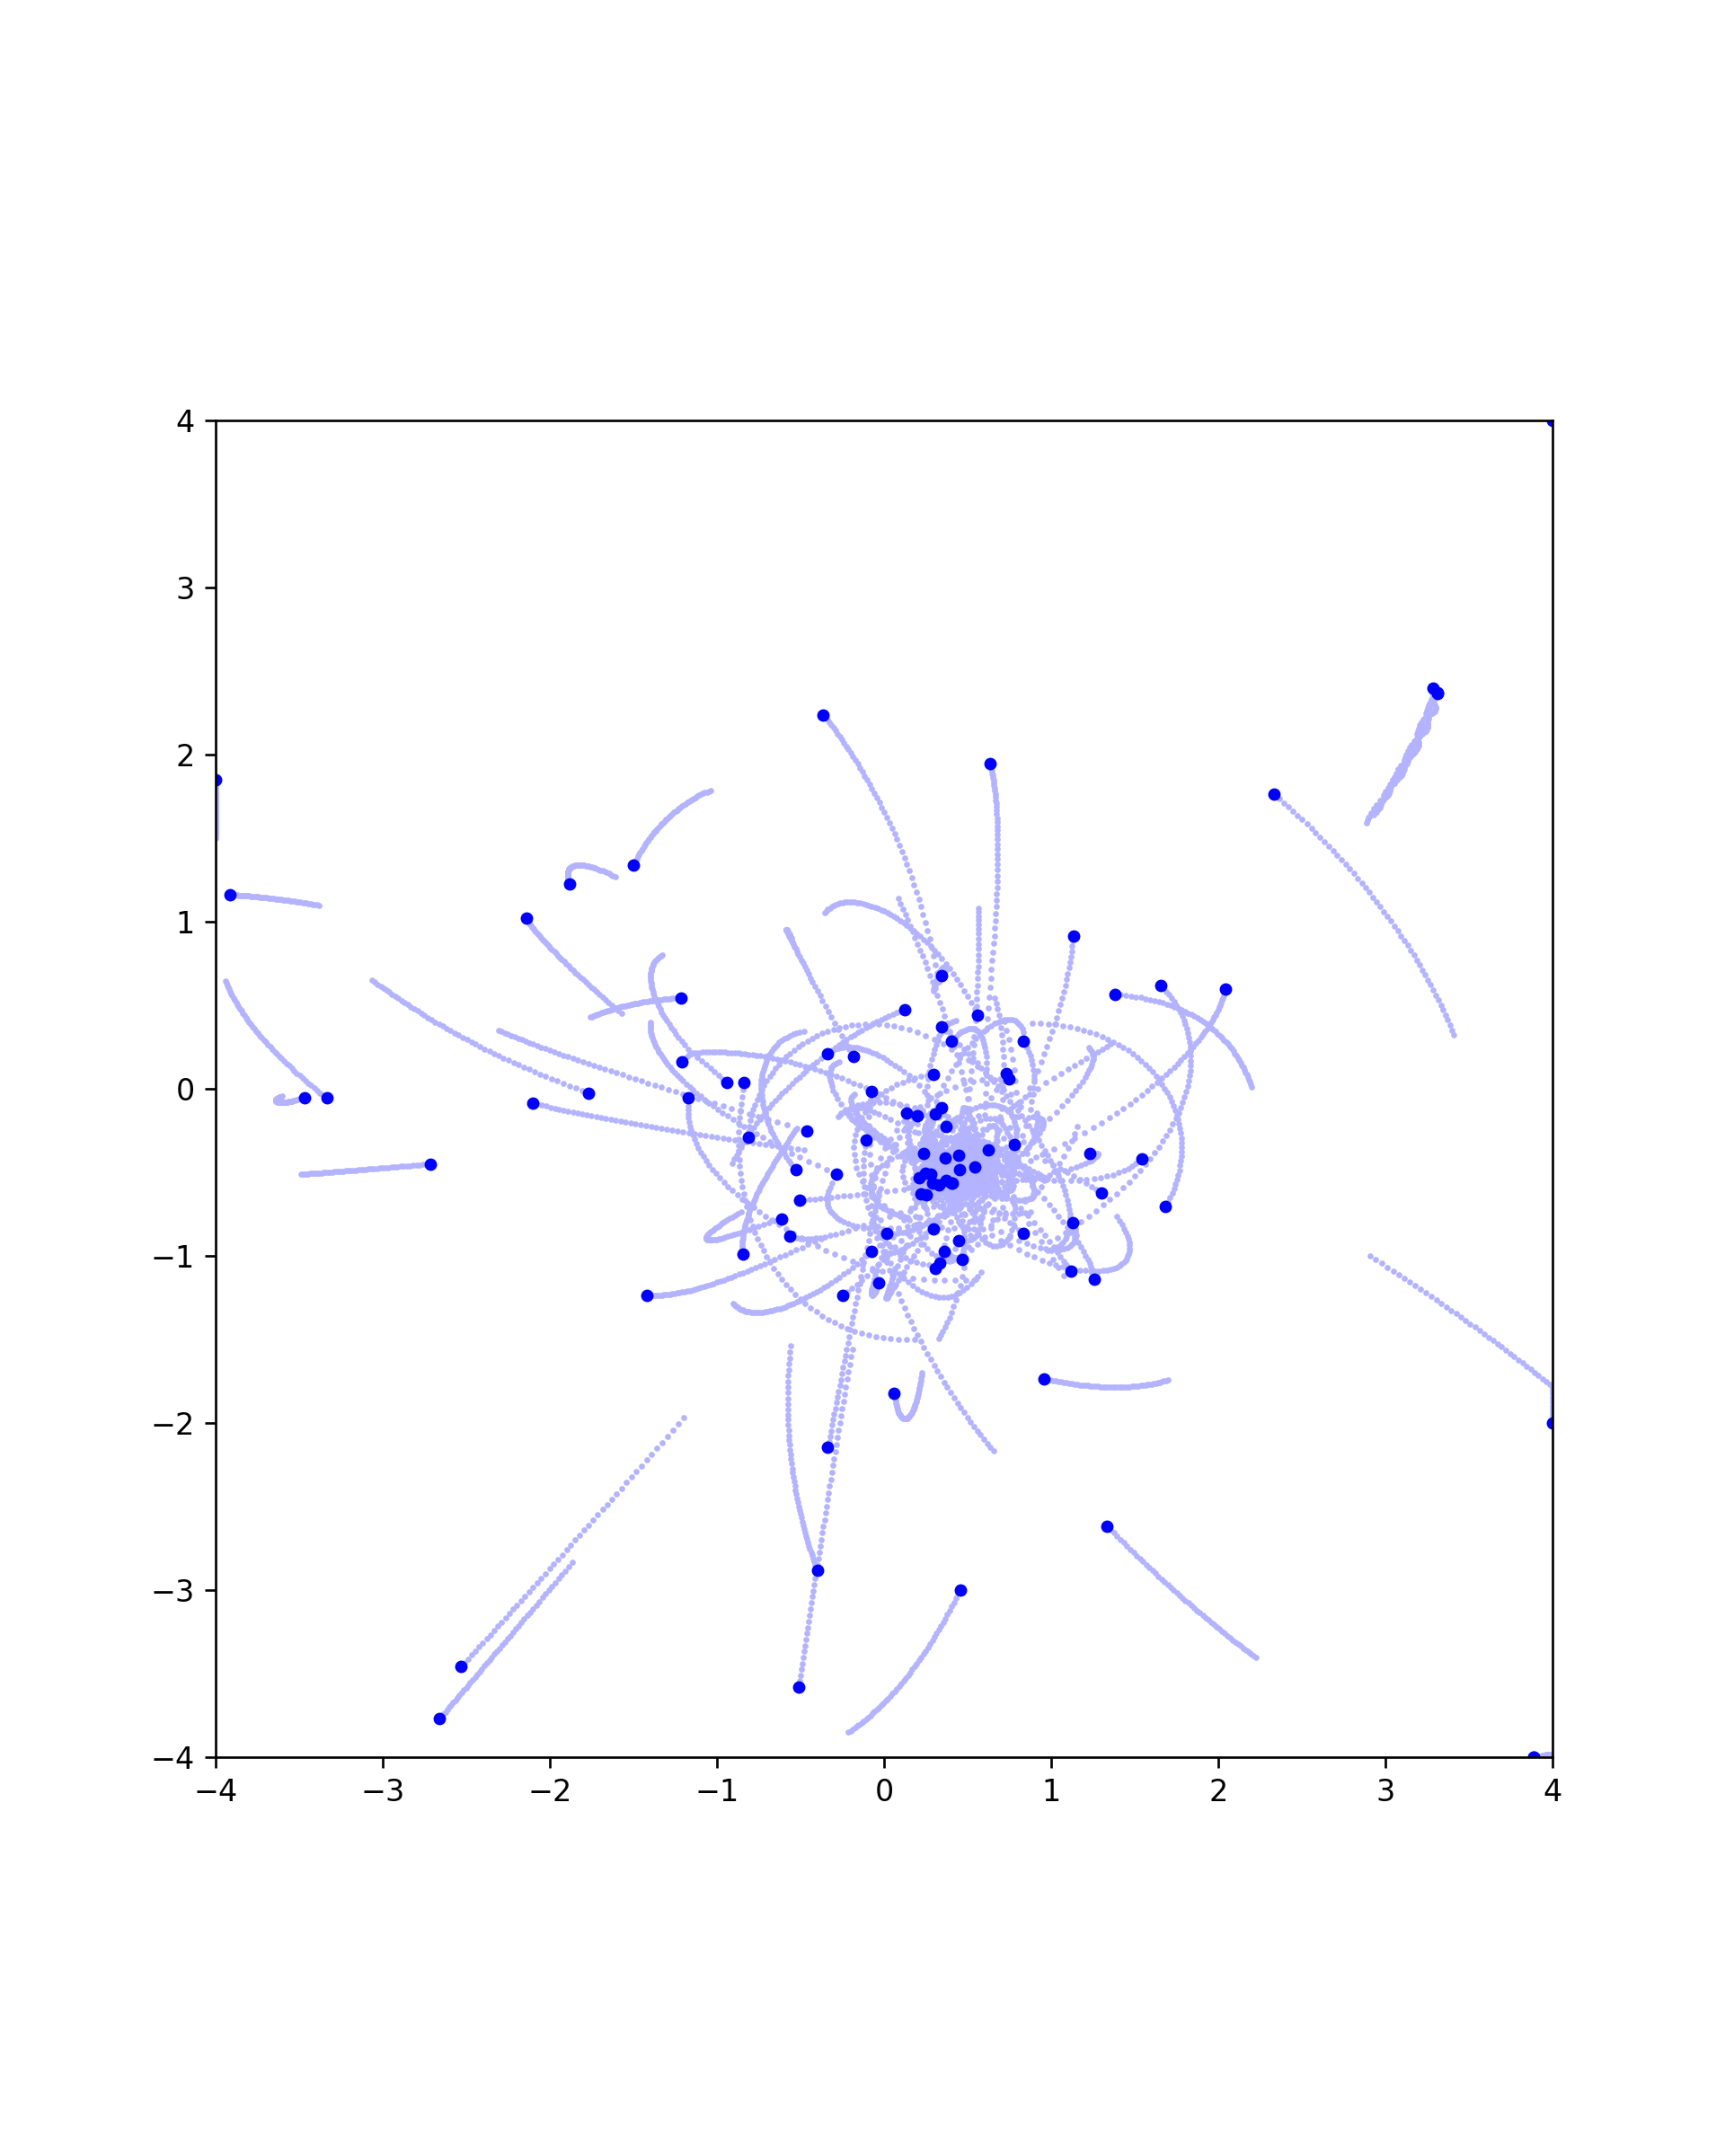
\includegraphics[width=0.4175\textwidth]{task1.png}
    \caption{Plot of the N-body simulation as computed by nbody.py}
\end{figure}
\newpage

\section{Question 2}

\subsection{}
\texttt{task2.cpp} can be found at \url{https://github.com/phantom3012/repo759/blob/main/HW04/task2.cpp} \\ \\
Plot of the positions is shown below:
\begin{figure}[ht]
    \centering
    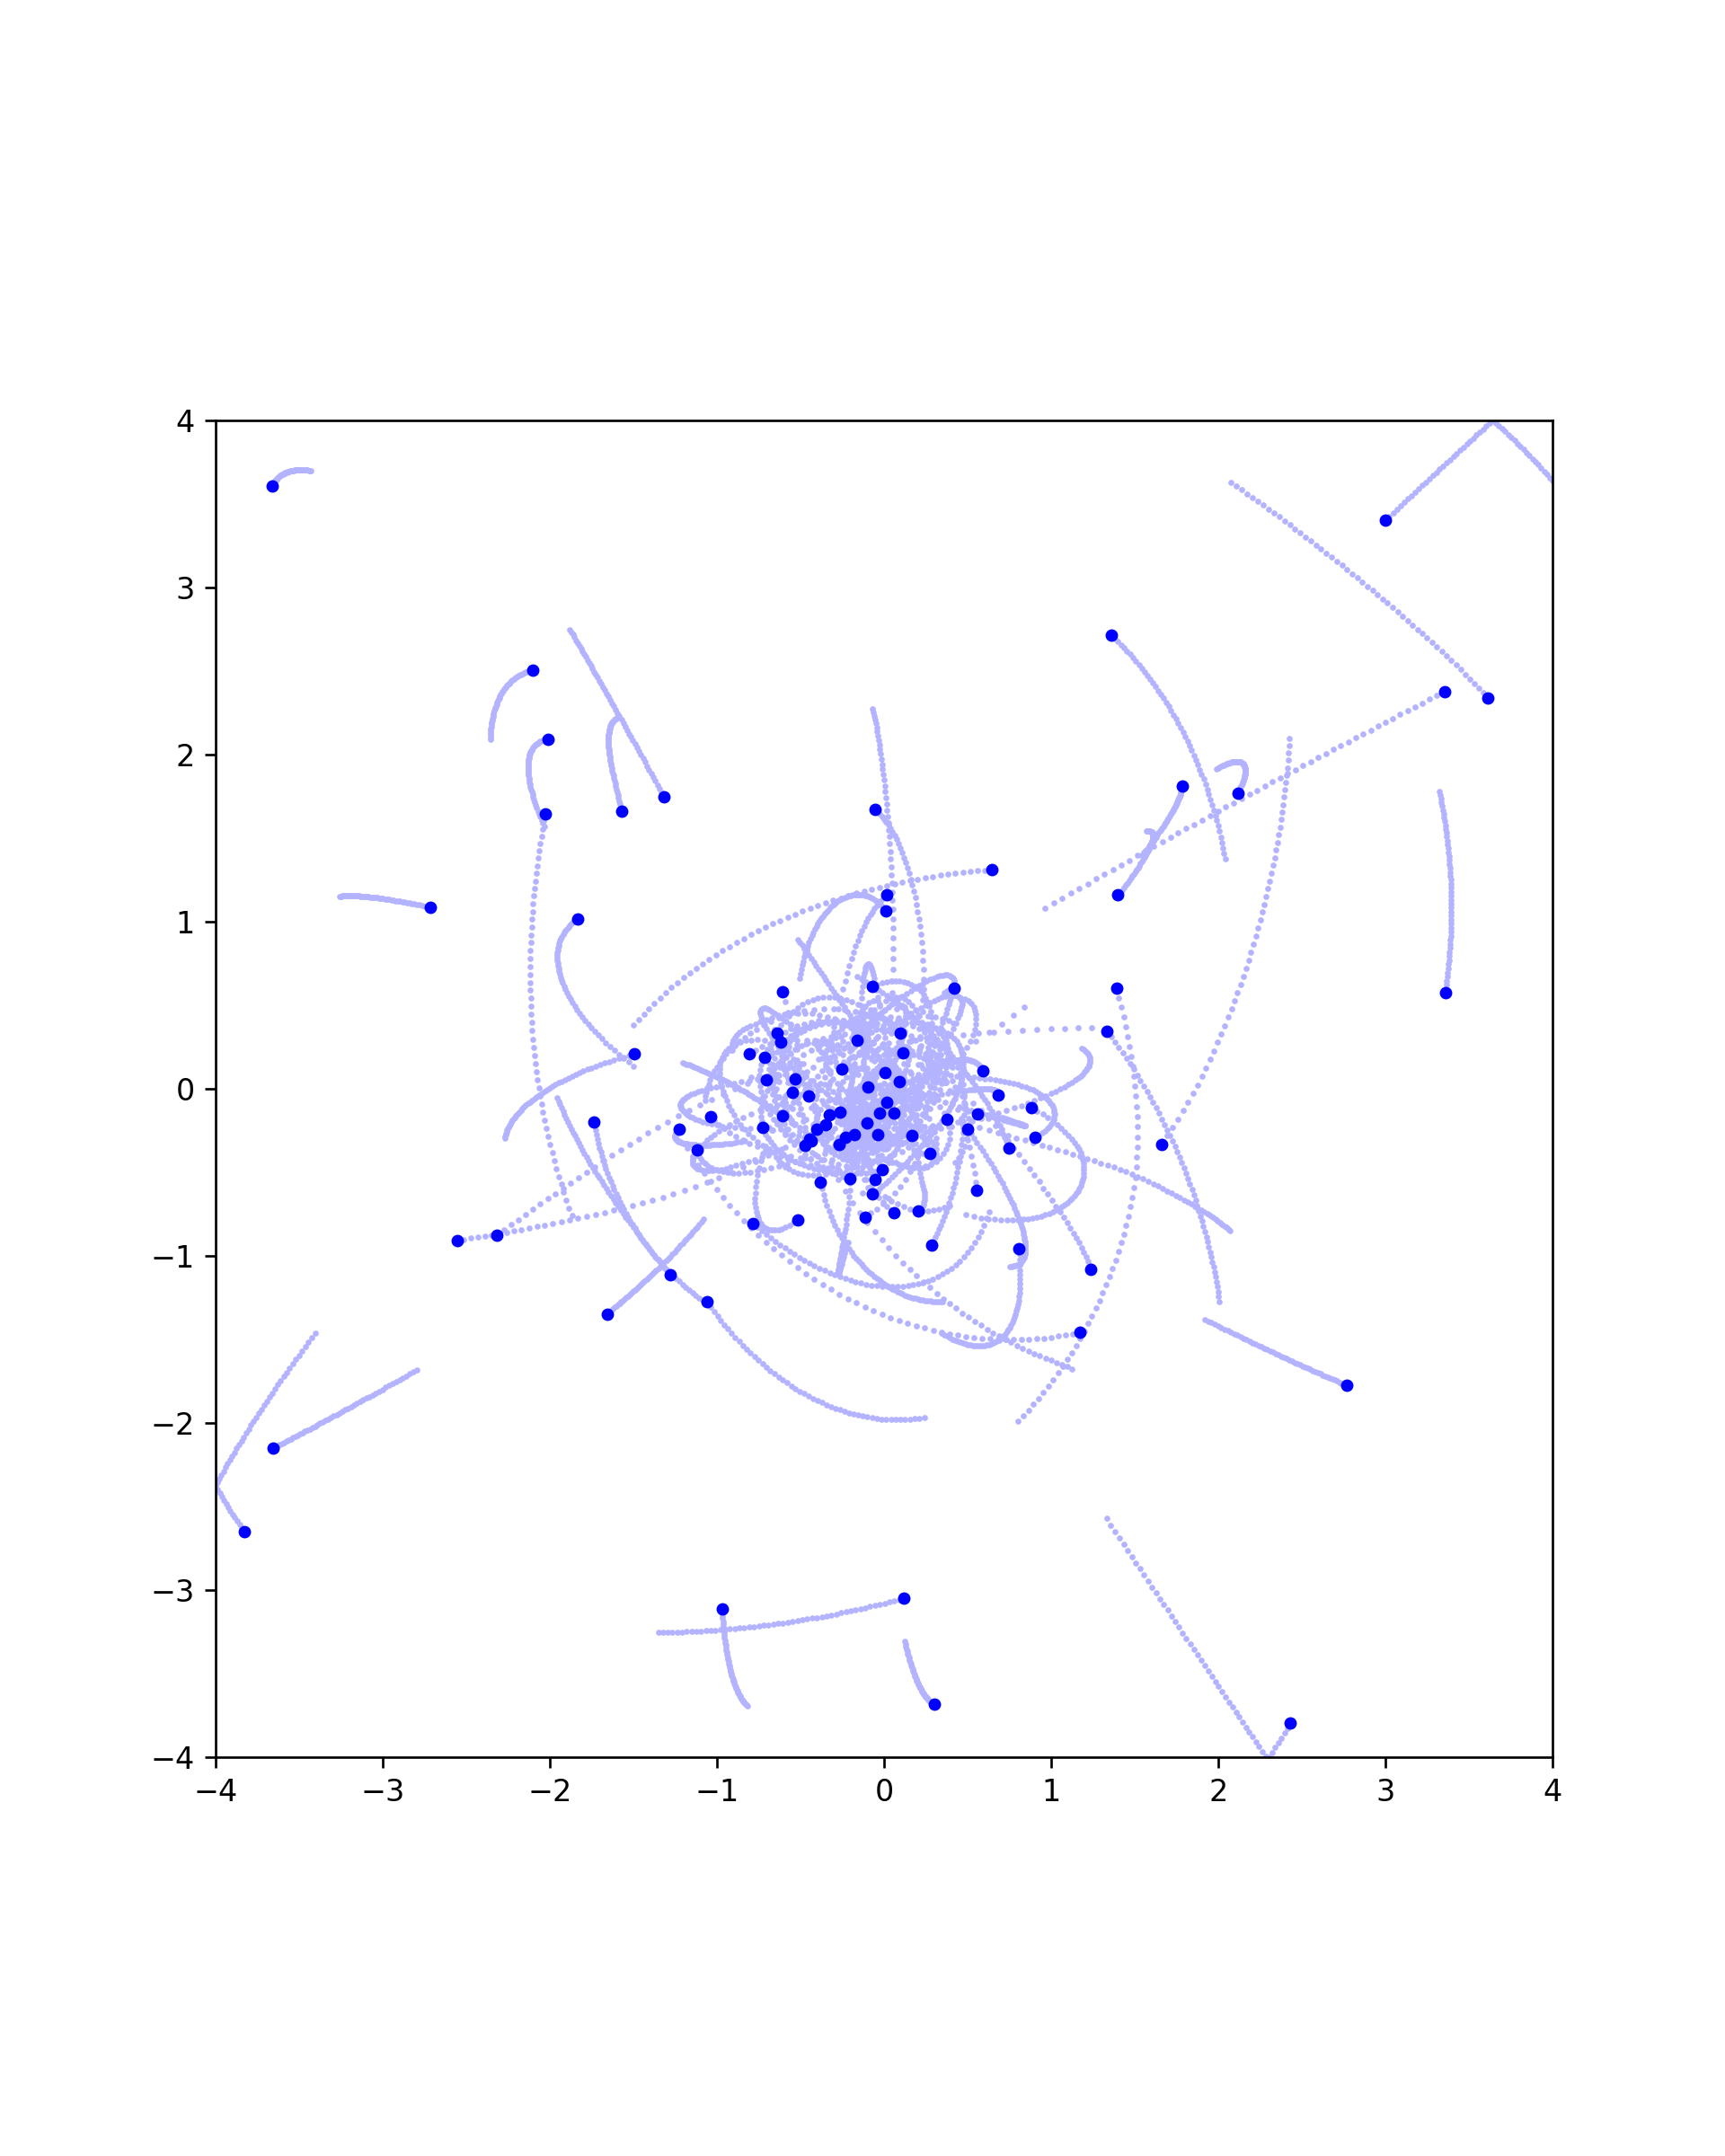
\includegraphics[width=0.5\textwidth]{nbody-cpp.png}
    \caption{Plot of the positions of the particles as generated by \texttt{plot\_positions.py}}
\end{figure}
\newpage
\section{Question 3}
\subsection{}
\texttt{task3.cpp} can be found at \url{https://github.com/phantom3012/repo759/blob/main/HW04/task3.cpp}

\section{Question 4}
\subsection{}
\texttt{task3.cpp} implemented with dynamic scheduling can be found at \url{https://github.com/phantom3012/repo759/blob/main/HW04/task4_dynamic.cpp} \\
\texttt{task3.cpp} implemented with guided scheduling can be found at \url{https://github.com/phantom3012/repo759/blob/main/HW04/task4_guided.cpp} \\
\texttt{task3.cpp} implemented with static scheduling can be found at \url{https://github.com/phantom3012/repo759/blob/main/HW04/task4_static.cpp} \\

\newpage
\subsection{}
\begin{figure}[ht]
    \centering
    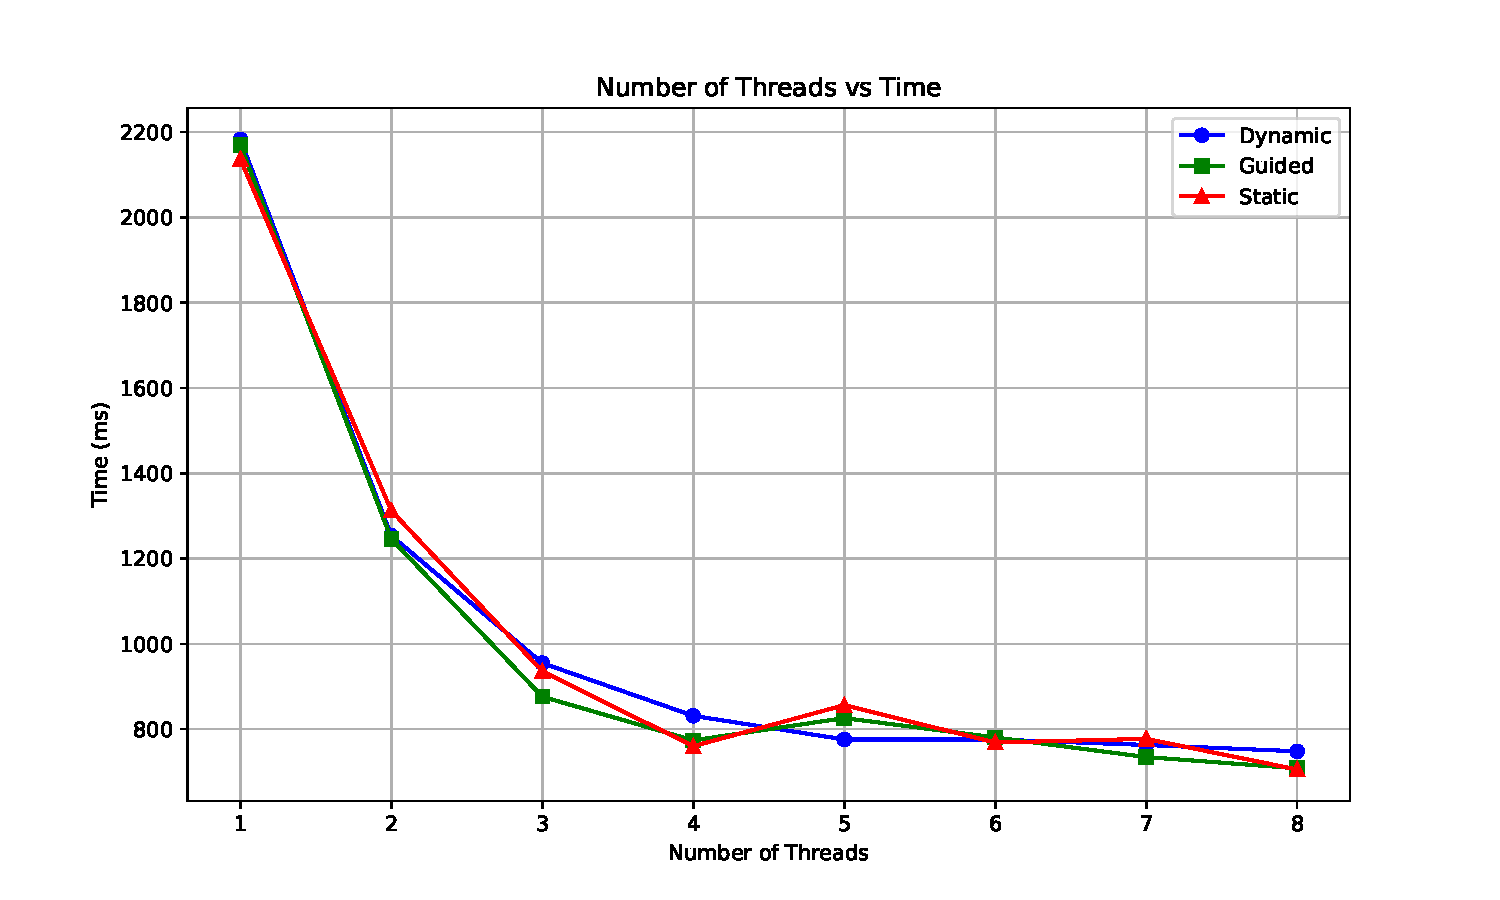
\includegraphics[width = \textwidth]{task4.pdf}
    \caption{Time taken vs. Number of threads for different scheduling types}
\end{figure}

\end{document}

